\chapter{Postestimation}\label{ch:postest}

After \texttt{nwdynam}, five \texttt{estat} commands work for every sub-model. They offer what \goldfish{} offers after estimation, with the same definitions and defaults: the log likelihood of every event (\texttt{returnIntervalLogL}), the model probabilities of the events (\texttt{returnEventProbabilities}), \texttt{logLik}, \texttt{AIC} and \texttt{BIC}, \texttt{examineOutliers} and \texttt{examineChangepoints}. \goldfish{} has no goodness-of-fit or simulation function, and \nwdynam{} adds none. The commands are evaluated at the coefficients in \texttt{e(b)} by the same native code as the fit.

The data of the fit is kept in memory after \texttt{nwdynam}. It is replaced by the next fit and gone after \texttt{clear all}, and the commands stop with return code 498 when the estimation results on screen are not those of the fit in memory (for example after \texttt{estimates restore} of an earlier fit; the message is shown in Section~\ref{sec:limits_estat}). Standard Stata postestimation (\texttt{estimates}, \texttt{lrtest}, \texttt{test}, \texttt{lincom}) works on the usual \texttt{e(b)} and \texttt{e(V)}.

\begin{lstlisting}
estat ic
estat eventlik   [, frame(name) replace]
estat eventprob  , frame(name) [replace maxrows(#)]
estat outliers   [, method(hampel|iqr|top) parameter(#) window(#) frame(name) replace plot name(name)]
estat changepoints [, moment(mean|variance) method(pelt|amoc|binseg) window(#) frame(name) replace plot name(name)]
\end{lstlisting}
The option \opt{frame(name)} stores the table in a new frame and \opt{replace} overwrites an existing frame. All examples of this chapter are in Section~\ref{sec:ex_post}.

\section{Information criteria}

\texttt{estat ic} reports the log likelihood, the log likelihood per event, AIC and BIC. It stores in \texttt{r()}: \texttt{r(ll)}, \texttt{r(ll\_per\_event)}, \texttt{r(N)} (the records of the log likelihood, as \goldfish{} counts them), \texttt{r(N\_events)} (the events), \texttt{r(df)}, \texttt{r(aic)}, \texttt{r(bic)} and the matrix \texttt{r(S)}. The BIC uses the number of events as the sample size. In the rate model with intercept the number of records is larger than the number of events (below), which \goldfish{} counts in the same way.

\section{The log likelihood of every event}

\texttt{estat eventlik} gives the log likelihood of every event: for the choice sub-model the log of the probability of the observed receiver; for the rate sub-model without intercept the log of the probability that the observed sender acts; for the coordination sub-model the log of the probability of the observed pair. It prints the number of events, the sum, the mean, the minimum and the maximum, and stores them as \texttt{r(N)}, \texttt{r(ll\_events)} (the sum over the events), \texttt{r(ll)}, \texttt{r(ll\_mean)}, \texttt{r(ll\_min)} and \texttt{r(ll\_max)}. With \opt{frame()} the table has the variables \texttt{event}, \texttt{origevent} (the row of the event in the data), \texttt{time}, \texttt{sender}, \texttt{receiver} and \texttt{ll}.

In the rate model \emph{with} intercept the log likelihood is a sum over the periods between events: besides one record per event, \goldfish{} includes the right-censored periods that a covariate change or the expiry of a window ends (they are part of \texttt{e(ll)}). The table then has one row per event and puts the censored periods before an event in the variable \texttt{llcens}; \texttt{r(n\_cens)} counts them and the part after the last event is in \texttt{r(ll\_trailing)}.

\section{The probabilities of the events}

\texttt{estat eventprob} gives the model probabilities of every event; because the table has one row per event and candidate it always needs \opt{frame()}. The variables are \texttt{event}, \texttt{time}, \texttt{actor} and \texttt{actorid} (\texttt{actor1}, \texttt{actor2} and their ids for the coordination sub-model), \texttt{observed} and \texttt{p}. The rows:
\begin{itemize}[nosep]
  \item choice: one row per event and candidate receiver, $p$ the probability that the actor is the receiver; the probabilities of an event sum to 1 over its candidates (with composition change or \opt{opportunities()} the candidates are those present or available);
  \item rate without intercept: one row per event and present actor, the probability that the actor is the sender;
  \item rate with intercept: for each actor \goldfish{} returns the linear predictor minus the exposure of the period that ends at the event; this is not a probability and is stored as \texttt{lnrate};
  \item coordination: one row per event and pair of actors (actor1 $<$ actor2); \texttt{p} is \goldfish{}'s matrix entry, twice the probability of the pair, so that the entries of an event sum to 1.
\end{itemize}
\opt{maxrows(\#)} limits the number of rows (events times candidates); the command stops with an error before it builds a larger table (default 200,000,000). \texttt{r(N\_rows)} and \texttt{r(frame)} are stored.

\section{Outliers}\label{sec:outliers}

\texttt{estat outliers} flags events whose log likelihood is unusually low, with the rules of \goldfish{}'s \texttt{examineOutliers}; \opt{method()}, \opt{parameter()} and \opt{window()} choose the rule.
\begin{description}[style=nextline,nosep]
  \item[\opt{method(hampel)}] (the default) flags an event whose log likelihood differs from the median of the \opt{window()} events on each side by more than \opt{parameter()} (default 3) scaled median absolute deviations. The default window is half the number of events minus 1, as in \goldfish{}, which tests only the middle event(s) of the log; give \opt{window()} for a rolling rule.
  \item[\opt{method(iqr)}] flags log likelihoods below the median minus \opt{parameter()}/2 interquartile ranges.
  \item[\opt{method(top)}] flags the \opt{parameter()} events with the lowest log likelihood. Events whose log likelihoods agree to the last digits are ranked in an arbitrary order, so that \goldfish{} may name another of them.
\end{description}
\opt{plot} draws the log likelihood against time with the flagged events marked; \opt{name()} names the graph. The command stores \texttt{r(n\_outliers)}, \texttt{r(N)}, \texttt{r(parameter)}, \texttt{r(window)}, \texttt{r(method)} and the row vector \texttt{r(outliers)} of the event numbers in increasing order; with \opt{frame()} the table has an indicator \texttt{outlier}. Figure~\ref{fig:outliers} shows the plot of the example.
\begin{figure}[ht]
\centering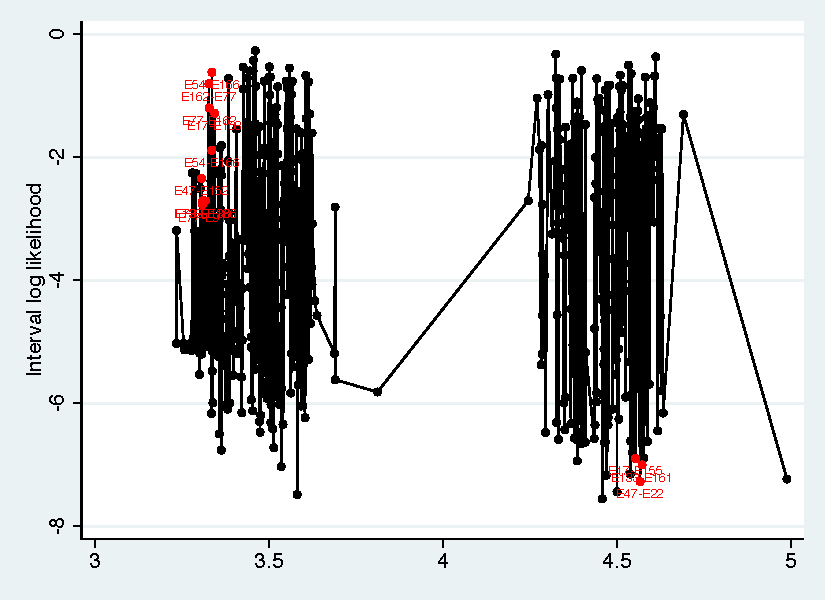
\includegraphics[width=0.8\textwidth]{fig/outliers.pdf}
\caption{\texttt{estat outliers, window(50) plot} after the choice model of Section~\ref{sec:ex_post}: the log likelihood of every event (the manufacturing emails), with the flagged events labelled sender--receiver.}\label{fig:outliers}
\end{figure}

\section{Change points}\label{sec:changepoints}

\texttt{estat changepoints} looks for regime changes in the log likelihood over the event sequence, with the methods of \goldfish{}'s \texttt{examineChangepoints}, which calls the R package \texttt{changepoint}. The methods are \opt{method(pelt)} (the default), \opt{method(amoc)} (at most one change) and \opt{method(binseg)} (binary segmentation, up to 5 changes), for the \opt{moment(mean)} (default) or the \opt{moment(variance)} of the log likelihood. \opt{window()} is the minimum segment length in events; the default is the largest number of events that share a time point, as in \goldfish{}. The penalty is the modified Bayesian information criterion and the test statistic is the normal one.

The change points are the events that end a regime: the log likelihood of the following events belongs to the next regime. The command stores \texttt{r(n\_cpts)}, \texttt{r(N)}, \texttt{r(window)}, \texttt{r(method)}, \texttt{r(moment)} and the row vector \texttt{r(cpts)} with the last event of every regime; the last entry is always the number of events, as in the R package. With \opt{frame()} the table has an indicator \texttt{cpt}.
\todoowner{\texttt{estat changepoints, plot} stopped with an error in a test for this manual (messages \texttt{\_\_000001 not found} and \texttt{time not found}, then \texttt{r(100)}; the program uses a matrix after it was returned by \texttt{return matrix}); without \texttt{plot} the command works. \texttt{estat outliers, plot} works. The help file documents \opt{plot} for both. Check, and either fix or leave the sentence out of this section.}

\paragraph{Credit.} The change point methods (PELT, AMOC and binary segmentation, for the mean and the variance of normal data, with a minimum segment length and the modified BIC penalty) are a port of the C code and of the penalty and cost functions of the R package \texttt{changepoint} (Rebecca Killick, Kaylea Haynes, Idris Eckley, Paul Fearnhead and Jamie Lee), so that \texttt{estat changepoints} gives the same change points as \goldfish{}.

\section{How the postestimation tools were checked}

Per-event log likelihoods and probabilities agree with \goldfish{} to 1e-13 on 90 random event logs (choice, rate, rate with intercept, coordination; with composition change, time-varying covariates, windows, two-mode networks, opportunities and effects of other networks); the outlier indices and the change points agree exactly (Chapter~\ref{ch:validation}).
